\chapter{Brass}\label{ch:brass}

\SWcomment[terms I could use: bore, tube, cylinder]

% In this work, the wave propagation in tubes is approximated using a 1D system.

Although not used for the contributions in Part \ref{part:contributions}, Webster's equation -- the 1D wave equation with a spatially varying cross-section -- will be presented. Then, Section \ref{sec:firstOrderSystem} decomposes Webster's equation into a system of two coupled first-order PDEs, which has been used to model the trombone in paper \citeP[H].


Unless denoted otherwise, this chapter follows \cite{theBible} and \cite{Bilbao2018}.

\section{Webster's Equation}\label{sec:webstersEq}
For an (axially symmetric) acoustic tube where the wavelengths of the frequencies at hand are much larger than the radius of the tube, one can simplify the system to be one-dimensional. For low-amplitude vibrations, one can describe the air propagation in this tube using \textit{Webster}'s equation \cite{Webster1919}
\begin{equation}\label{eq:webstersPDE}
    S\partial_t^2\Psi = c^2\partial_x(S\partial_x\Psi),
\end{equation}
with \textit{acoustic potential} $\Psi = \Psi(x,t)$ (in m$^2$/s), the cross-sectional area along the tube, or bore profile $S = S(x)$ (in m$^2$) and the speed of sound in air $c$ (in m/s). If $S(x)$ is constant, Eq. \eqref{eq:webstersPDE} reduces to the 1D wave equation in Eq. \eqref{eq:1DwavePDE}. For a tube of length $L$ (in m), $\Psi$ is defined for $x \in \D$ where domain $\D = [0, L]$. The acoustic potential can be related to pressure $p = p(x,t)$ (in Pa) and particle velocity $v = v(x,t)$ (in m/s) according to \cite{Bilbao2018}
\begin{equation}
    p = \rho \pt \Psi, \qaq v = -\px \Psi.
\end{equation}

\subsection{Boundary Conditions}
The choices for boundary conditions in an acoustic tube are open and closed, defined as \cite{Bilbao2018}
\begin{subequations}\label{eq:contBoundariesBrass}
    \begin{align}
        \partial_t\Psi &= 0\quad \text{(Dirichlet, open)}\label{eq:contDirichletBrass}\\
        \partial_x\Psi &= 0\quad \text{(Neumann, closed)}\label{eq:contNeumannBrass},
    \end{align}
\end{subequations} 
at the ends of the tube. This might be slightly counter-intuitive as in the case of a string ``closed" might imply the ``fixed" or Dirichlet boundary condition. The opposite can be intuitively shown imagining a wave front with a positive acoustic potential moving through a tube and hitting a closed end. What reflects is also a wave front with a positive acoustic potential, i.e., the sign of the potential does not flip, which also happens using the free or Neumann condition for the string (see Figure \ref{fig:boundaryCondsCont}).
In this work the following boundaries are chosen
\begin{equation}\label{eq:openClosed}
    \partial_x\Psi(0, t) = 0, \quad \text{and} \quad \partial_t\Psi(L, t) = 0,
\end{equation}
i.e. closed at the left end and open at the right end.

\section{Discrete Time}
The state variable is discretised to the grid function $\Psi_l^n$ and is defined for $n\in \mathbb{N}^0$ and $l = \{0, \hdots, N\}$, where $N$ is the number of intervals between the grid points.
As the cross-section is distributed along space $x$, $S(x)$ needs to be discretised to a grid function as well, albeit only in space. Following \cite{Bilbao2018}, it is useful to introduce \textit{interleaved grid points} at $l-1/2$ and $l+1/2$ for $S$ and are defined as 
\begin{equation}\label{eq:sHalf}
    \Sm = \mxm S(x=lh), \qaq \Sp = \mxp S(x=lh),
\end{equation}
and approximate a `true' (or possibly measured) bore profile $S(x)$ sampled at $x=lh$ with grid spacing $h$. Using these definitions, one can discretise Eq. \eqref{eq:webstersPDE} to the following FD scheme \cite{Bilbao2018}
\begin{equation}\label{eq:discWebster}
    \Sbar_l \delta_{tt}\Psi^n_l = c^2\dxp(\Sm(\delta_{x-}\Psiln)),
\end{equation}
where
\begin{equation}\label{eq:Sbar}
    \Sbar_l = \mxp\Sm = \mxx S(x=lh),
\end{equation}
the choice of which will be come apparent in Section \ref{}
See Figure \ref{fig:variableCrossSection}.
The right-hand side of the scheme contains an operator applied to two grid functions ($S$ and $\Psi$) multiplied onto each other. In order to expand this, the product rule must be used. Recalling Eq. \eqref{eq:productRule} and applying this to spatial operators instead yields
\begin{equation}
    \dxp (u_l^nw_l^n) = (\dxp u_l^n)(\mxp w_l^n) + (\mxp u_l^n)(\dxp w_l^n).
\end{equation}
Using the product rule, the right-hand side of Eq. \eqref{eq:discWebster} can be expanded to
\begin{equation*}
    \Sbar\dtt\Psiln = c^2\left[(\dxp \Sm)(\mxp (\dxm \Psiln)) + (\mxp \Sm)(\dxp (\dxm \Psiln))\right]
\end{equation*}
and solving for $\Psinp$ yields the following update equation:
\begin{equation}
    \Psinp = 2(1-\lambda^2)\Psiln-\Psinm+ \frac{\lambda^2\Sp}{\Sbar_l}\Psilp + \frac{\lambda^2\Sm}{\Sbar_l}\Psilm,\label{eq:webstersUpdateEq}
\end{equation}
with 
\begin{equation}
    \lambda = \frac{ck}{h}
\end{equation}
and similar to the 1D wave equation in Section \ref{sec:1DWaveDisc}
\begin{equation}
    \lambda \leq 1,
\end{equation}
in order for the scheme to be stable. 

Notice that at the boundaries, Eq. \eqref{eq:webstersUpdateEq} requires values of $S$ (through its definition in Eq. \eqref{eq:Sbar}) outside of the defined domain, i.e., $S_{N+1/2}$ and $S_{-1/2}$. To solve this, one can set $\Sbar_0 = S(0)$ and $\Sbar_N = S(L)$ from which $S_{-1/2}$ and $S_{N+1/2}$ can be calculated according to
\begin{subequations}
    \begin{align}
        \Sbar_0 = \frac{1}{2}(S_{1/2} + S_{-1/2}) \ &\Rightarrow \ S_{-1/2} = 2\Sbar_0 - S_{1/2},\\
        \Sbar_N = \frac{1}{2}(S_{N+1/2} + S_{N-1/2}) \ &\Rightarrow \ S_{N+1/2} = 2\Sbar_N - S_{N-1/2}.\label{eq:Snph}
    \end{align} 
\end{subequations}
\begin{figure}[t]
    \centering
    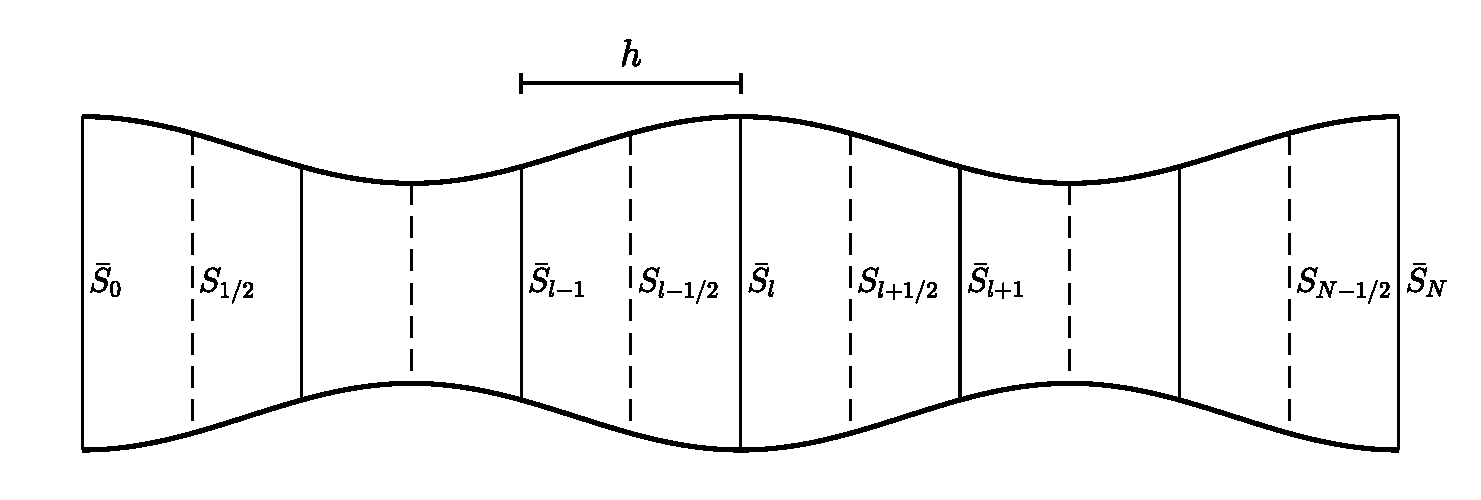
\includegraphics[width=0.9\textwidth]{figures/resonators/brass/variableCrossSection.eps}
    \caption{Approximations to $S(x)$ used in the FD scheme implementing Webster's equation. Dashed lines indicate the interleaved grid on which $S$ is sampled according to Eq. \eqref{eq:sHalf}. \label{fig:variableCrossSection}}
\end{figure}
Although these values will not be needed when discretising the boundary conditions in Eq. \eqref{eq:contBoundariesBrass}, they will be useful at a later point.

\subsection{Boundary Conditions}
One can discretise the continuous boundary conditions in Eq. \eqref{eq:openClosed} (closed at $x=0$, open at $x=L$) using centred difference operators for higher accuracy
\begin{subequations}\label{eq:discBoundariesBrass}
    \begin{align}
        \dxd\Psi_0^n &= 0 \quad \Rightarrow \quad\Psi_{-1}^n = -\Psi_1^n \quad \!\!\!\!\!\!&&\text{(Neumann, closed)} \label{eq:closedLeftBrass}\\
        \dtd\Psi_N^n &= 0\quad\Rightarrow \quad \Psi_N^n = 0 \quad \!\!\!\!\!\!&&\text{(Dirichlet, open)}\label{eq:openRightBrass}.
    \end{align}
\end{subequations} 
At the left boundary, Eq. \eqref{eq:webstersUpdateEq} can be expanded to:
\begin{equation*}
    \begin{aligned}
        \Psi_0^{n+1} &= 2(1-\lambda^2)\Psi_0^n-\Psi_0^{n-1}+ \frac{\lambda^2S_{1/2}}{\bar S_0}\Psi_1^n + \frac{\lambda^2S_{-1/2}}{\bar S_0}\Psi_{-1}^n,\\[-0.5em]
        \xLeftrightarrow{\mystrut\ \text{Eq. \eqref{eq:closedLeftBrass}}\ }\quad\Psi_0^{n+1} &= 2(1-\lambda^2)\Psi_0^n-\Psi_0^{n-1}+ \frac{\lambda^2(S_{1/2}+S_{-1/2})}{\bar S_0}\Psi_1^n,
    \end{aligned}
\end{equation*}
and as $\Sbar_0 = \frac{1}{2}(S_{1/2}+S_{-1/2})$ through Eq. \eqref{eq:Sbar} can be solved to
\begin{equation}
    \Psi_0^{n+1} = 2(1-\lambda^2)\Psi_0^n-\Psi_0^{n-1}+ 2\lambda^2\Psi_1^n.
\end{equation}
One can implement the right boundary condition by simply reducing the range of operation to $l = \{0, \hdots, N-1\}$, as $\Psi_N^n = 0$ according to Eq. \eqref{eq:openRightBrass}. A more realistic boundary condition for the open end is presented in the following.

\subsection{Radiation}\label{sec:radiating}
One of the ways that brass instruments lose energy, is through radiation. The right boundary condition presented in Eq. \eqref{eq:openClosed} can be changed to be radiating according to \cite{theBible}
\begin{equation}\label{eq:radCont}
    \partial_x\Psi(L,t) = -a_1\partial_t\Psi(L,t)-a_2\Psi(L,t),
\end{equation}
where for a tube terminating on an infinite plane \cite{Atig2004}
\begin{equation}
    a_1 = \frac{1}{2(0.8216)^2c} \quad \text{and} \quad a_2 = \frac{L}{0.8216\sqrt{S_0S(1)/\pi}},
\end{equation}
which determine the amount of loss and inertia respectively. 

The radiating boundary in Eq. \eqref{eq:radCont} can then be discretised to \cite{theBible}
\begin{equation}\label{eq:centRadBound}
    \delta_{x\cdot}\Psi_N^n = -a_1\dtd\Psi_N^n - a_2\mu_{t\cdot}\Psi_N^n.
\end{equation}
This can be expanded and solved for $\Psi_{N+1}^n$ according to
\begin{equation}
    \Psi_{N+1}^n = h\left(-\frac{a_1}{k}(\Psi_N^{n+1} - \Psi_N^{n-1}) - a_2(\Psi_N^{n+1} + \Psi_N^{n-1})\right) + \Psi_{N-1}^n,
\end{equation}
and substituted into Eq. \eqref{eq:webstersUpdateEq} at the right boundary to get the following update equation
\begin{equation}
    \Psi_N^{n+1} = \frac{2(1-\lambda^2)\Psi_N^n-\Psi_N^{n-1}+\frac{h\lambda^2S_{N+1/2}}{\bar S_N}\left(\frac{a_1}{k}-a_2\right)\Psi_N^{n-1} + 2\lambda^2\Psi_{N-1}^n}{\left(1+\left(\frac{a_1}{k}+a_2\right)\frac{h\lambda^2S_{N+1/2}}{\bar S_N}\right)}.
\end{equation}
One can observe that an value for the  cross-sectional outside the defined domain is needed. As mentioned before, setting $\Sbar_N = S(L)$, one can calculate $S_{N+1/2}$ using Eq. \eqref{eq:Snph} solving the issue. 

% At the left boundary, one can sed $\bar S_N = S_N$ from which $S_{N+1/2}$ can be calculated:
% \begin{equation}
%     S_N = \frac{1}{2}(S_{N+1/2} + S_{N-1/2}) \ \Rightarrow \ S_{N+1/2} = 2S_N - S_{N-1/2}.
% \end{equation}
% % \begin{equation}
% %         S_0 = \frac{1}{2}(S_{1/2} + S_{-1/2}) \ \Rightarrow \  S_{-1/2}
% %         = 2S_0 - S_{1/2}
% % \end{equation}



% The same can be done for the right boundary ($\bar S_N = S_N$) if this is chosen to be anything else but open (e.g., closed or radiating -- see Section \ref{sec:radiating}):
% \begin{equation}
%     S_N = \frac{1}{2}(S_{N+1/2} + S_{N-1/2}) \ \Rightarrow \ S_{N+1/2} = 2S_N - S_{N-1/2}.
% \end{equation}
% For now though, we follow the conditions given in \eqref{eq:openClosed} and we can simply set the right boundary to its initial state
% \begin{equation}
%     \Psi_N^n = \Psi_N^0
% \end{equation}
% which is normally $0$. A more realistic open end is a radiating one, which can be found below.

\subsection{Output and Matrix Form}

\begin{equation}
    \Dxx = \frac{1}{h^2}\begin{bmatrix}
        -2& 2 &  & & & \mathbf{0}& \\
        \frac{S_{1/2}}{\Sbar_1} & -2 &\frac{S_{3/2}}{\Sbar_1} & & & & \\
        & \ddots & \ddots & \ddots &  & & \\
        & & \frac{S_{l-1/2}}{\Sbar_l}& -2 & \frac{S_{l+1/2}}{\Sbar_l} & & \\
        & & & \ddots & \ddots & \ddots & \\
        & & &  & \frac{S_{N-3/2}}{\Sbar_{N-1}}  & -2 & \frac{S_{N-1/2}}{\Sbar_{N-1}} \\
        & \mathbf{0} & & & & 2 & -2 \\
    \end{bmatrix}.
\end{equation}

\subsection{Energy Analysis}
Energy analysis of Webster's equation with a radiating end might seem straightforward. However, due to the varying cross-sectional area, the energy balance deserves a more detailed treatment. Especially the boundaries become difficult to handle. For this analysis, (centred) Neumann boundary conditions are used for both boundaries to retain generality. %These can then easily be adapted to Dirichlet if needed.

\subsubsection{Step 1: Obtain $\dtp \h$}
To obtain the proper boundary terms when using centred Neumann boundary conditions, the primed inner product in Eq. \eqref{eq:primedInnerProd} can usually be chosen. However, as the system has a varying cross-section, the more general \textit{weighted inner product} in Eq. \eqref{eq:weightedInnerProd} has to be chosen instead.

Taking an inner product weighted by free parameters $\el, \er > 0$ at the left and right boundary respectively, of scheme \eqref{eq:discWebster} with respect to $(\dtd \Psiln)$ over discrete domain $d$ yields 
\begin{equation}\label{eq:powerBalanceWebster}
    \dtp \h = \langle \dtd\Psiln ,\Sbar_l \delta_{tt}\Psi^n_l\rangle_d^{\el,\er} - c^2\langle\dtd\Psiln, \dxp(\Sm(\delta_{x-}\Psiln))\rangle_d^{\el,\er} = 0.
\end{equation}

\subsubsection{Step 2: Identify energy types and isolate $\dtp$} 
As the right boundary is set to be radiating according to Eq. \eqref{eq:centRadBound} the energy balance will be of the following form:
\begin{equation}\label{eq:radiatingEnergyForm}
    \delta_{t+}(\mathfrak{h}+\mathfrak{h}_\text{b}) = \b-\mathfrak{q}_\text{b},
\end{equation}
where $\mathfrak{h}_\text{b}$ is the energy stored by the boundary through the inertia term, $\mathfrak{q}_\text{b}$ are the energy losses and $\b$ is the boundary term.

It can be shown that
\begin{equation}
    \dxp\left(\Sm(\delta_{x-}\Psiln)\right) \ \Longleftrightarrow\  \dxm\big(\Sp(\dxp\Psiln)\big),
\end{equation}
i.e. changing the signs of the operators at the right hand side. Then, using identities \eqref{eq:prodIdentity1} for the first term and \eqref{eq:weightedIdentityMinus} for the second yields (notice that $\b_\text{l}$ is subtracted)
\begin{equation*}
    \dtp \h = \b_\text{r} - \b_\text{l}
\end{equation*}
where
\begin{equation}
    \begin{gathered}
        \h = \t + \v, \qwiq \t = \frac{1}{2} \left(\lVert\sqrt{\Sbar_l} \dtm \Psiln \rVert_d^{\el, \er}\right)^2 \quad \text{and} \\
        \v =c^2\langle\dtd \dxp \Psiln, \Sp(\dxp \Psiln)\rangle_{\underline{d}}\ .
    \end{gathered}
\end{equation}
Notice that $\Sbar_l$ is included in the norm by using its square-root. Moreover,
\begin{subequations}
\begin{align}
 \mathfrak{b}_\text{r} &= c^2(\dtd\Psi_N^n)\left(\frac{\epsilon_\text{r}}{2}S_{N+1/2}(\dxp \Psi_N^n) + \left(1-\frac{\epsilon_\text{r}}{2}\right)S_{N-1/2}(\dxm\Psi_N^n)\right), \\
 \mathfrak{b}_\text{l} &= c^2(\dtd\Psi_0^n)\left(\frac{\epsilon_\text{l}}{2}S_{-1/2}(\dxm\Psi_0^n)+\left(1-\frac{\epsilon_\text{l}}{2}\right)S_{1/2}(\dxp \Psi_0^n))\right),
\end{align}
\end{subequations}
are the right and left boundary term respectively. Notice that if Dirichlet boundary conditions would be used, the boundary terms vanish. 

If (centred) Neumann conditions are used instead, the goal is now to find definitions for $\el$ and $\er$ such that the boundaries are strictly dissipative. In other words, if the boundary terms can be rewritten to $(\dxd \Psi_0^n) = 0$ or $(\dxd \Psi_N^n) = 0$ for the left and right boundary, respectively, this would achieve the goal. It can be shown that, for the special cases of $\epsilon_\text{r} = S_{N-1/2}/\mu_{xx}S_N$ and $\epsilon_\text{l} = S_{1/2}/\mu_{xx}S_0$ the boundary terms become strictly dissipative 
\begin{subequations}\label{eq:centStrictDissip}
\begin{align}
    \mathfrak{b}_\text{r} &= c^2 (\dtd\Psi_N^n)S_{N-1/2}(2-\epsilon_\text{r})(\delta_{x\cdot}\Psi_N^n)\label{eq:centStrictDissipRight},\\
    \mathfrak{b}_\text{l} &= c^2 (\dtd\Psi_0^n)S_{1/2}(2-\epsilon_\text{l})(\delta_{x\cdot}\Psi_0^n).\label{eq:centStrictDissipLeft}
\end{align}
\end{subequations}
One can then include the radiation at the right boundary by substituting its definition from Eq. \eqref{eq:centRadBound} into \eqref{eq:centStrictDissipRight} to get
\begin{align*}
    \mathfrak{b}_\text{r} &= c^2 (\dtd\Psi_N^n)S_{N-1/2}(2-\epsilon_\text{r})(-a_1\dtd\Psi_N^n - a_2\mu_{t\cdot}\Psi_N^n),\\
    &= c^2 S_{N-1/2}(2-\epsilon_\text{r})\left(-a_1(\dtd\Psi_N^n)^2 - a_2(\dtd\Psi_N^n)(\mu_{t\cdot}\Psi_N^n)\right),
\end{align*}
and using identites \eqref{eq:prodIdentity4} -- and \eqref{eq:identity2} thereafter -- yields the definitions for $\h_\text{b}$ and $\q_\text{b}$ in Eq. \eqref{eq:radiatingEnergyForm}
\begin{equation}
    \h_\text{b} = \frac{c^2 S_{N-1/2}(2-\epsilon_\text{r}) a_2}{2} \mtm(\Psi_N^n)^2, \qaq \q_\text{b} = c^2 S_{N-1/2}(2-\epsilon_\text{r})a_1(\dtd\Psi_N^n)^2.
\end{equation}

\subsubsection{Step 3: Check units}
\SWcomment[It seems like in order for the units to make sense, one must write Eq. \eqref{eq:webstersPDE} as
\begin{equation}
    \frac{S\rho}{c^2} \ptt\Psi = \frac{B}{c^2}\px(S(\px\Psi)),
\end{equation}
where $B$ is the bulk modulus of air (in N/m$^2$)]
\subsubsection{Step 4: Implementation}
Figure \ref{fig:energyWebsters} shows the energetic output of Webster's equation with a radiating boundary at $x=L$. The system is excited with a raised cosine close to the left boundary, and when the excitation reaches the radiating boundary, the total energy in the system decreases due to the losses.
\begin{figure}[h]
    \centering
    \begin{tikzpicture}[->,node distance=3cm,
        thick,main node/.style={circle,draw}]
    
        \node[] (image) at (0,0) {
        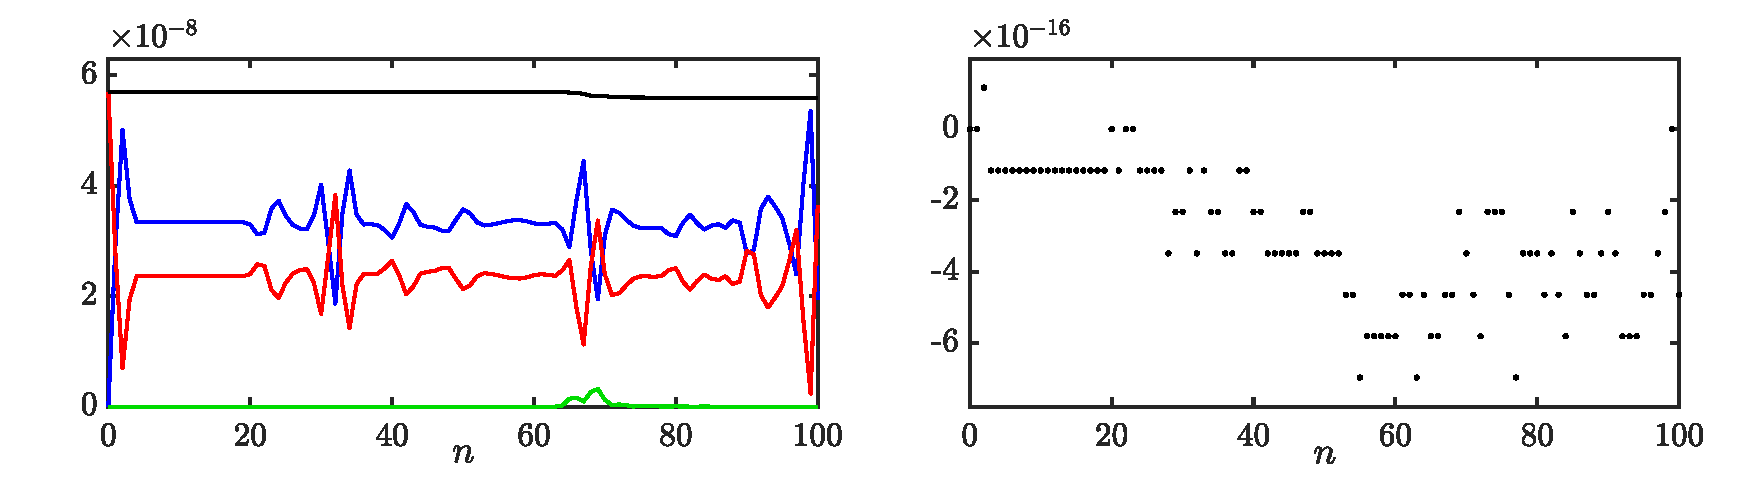
\includegraphics[width=\textwidth]{figures/resonators/brass/energyWebster.eps}
        };
    
        \node[] (he) at (0.2,0.5) {\small $\mathfrak{h}_\text{e}$};

        \node[] (h) at (-5.75, 1) {\small $\mathfrak{h}$};
        \node[] (v) at (-5.75, 0.5) {\small $\color{red}\mathfrak{v}$};
        \node[] (t) at (-5.75, 0) {\small $\color{blue}\mathfrak{t}$};
        \node[] (hb) at (-5.75, -0.5) {\small $\color[HTML]{00DB00}\mathfrak{h}_\text{b}$};      
    \end{tikzpicture}
      \caption{The kinetic (blue), potential (red), and total (black) energy as well as the energy stored by the radiation condition (green) of an implementation of Webster's equation are plotted in the left panel. Notice that the energy decreases around $n=65$ as the excitation reached the boundary where damping is included. The right panel shows the normalised energy (according to Eq. \eqref{eq:normalisedEnergyDamping}) and shows that the deviation of the energy is within machine precision. \label{fig:energyWebsters}}
\end{figure}

\subsection{Stability through Energy Analysis}
Frequency domain analysis as presented in Section \ref{sec:stabilityAnalysis}, or more specifically, von Neumann analysis, can not be performed on Webster's equation as the system has a varying cross-section \cite{theBible}. Instead, stability conditions can be obtained through energy analysis explained in Section \ref{sec:stabilityAnalysisEnergy}.



\section{First-order system}\label{sec:firstOrderSystem}
Until now, the only PDEs presented have been second-order in time, i.e., are dependent on the acceleration of the state variable. This section presents a system of two coupled first-order PDEs which has been used to model the trombone in paper \citeP[H]. second-order PDE  These equations are dependent on 

This will be the first appearance of a first-order system. 



\subsection{Adding Radiation}
\def\r{\text{r}}
\def\one{{(1)}}
Following \cite{Harrison2018} we can add a radiation to the schemes using a circuit representation of the Levine and Schwinger radiation model \SWcomment[(See Figure \textbackslash ref\{fig:radiation\})]. The system can be described as
\begin{subequations}\label{eq:barVPSystem}
    \begin{align}
        \bar v &= \mu_{t+}v_\one + \frac{1}{R_2}\mu_{t+}p_\one + C_\r \delta_{t+}p_\one,\label{eq:barV}\\
        \bar p &= L_\r \delta_{t+}v_\one,\label{eq:barP1}\\
        \bar p &= \left(1+\frac{R_1}{R_2}\right)\mu_{t+}p_\one+ R_1 C_\r\delta_{t+}p_\one\label{eq:barP2},
    \end{align}
\end{subequations}
where $\bar p^{n+1/2}$ and $\bar v^{n+1/2}$ lie on the interleaved temporal grid and are related to the tube by
\begin{equation}\label{eq:barVars}
    \bar p = \mu_{t+}p^n_N, \quad \bar S_N \bar v = \mu_{x-}\left(S_{N+1/2}v_{N+1/2}^{n+1/2}\right).
\end{equation}
We can couple this to the tube by taking Eq. \eqref{eq:pressureUpdate} at $l = N$
\begin{equation}
    p_N^{n+1} = p_N^n - \frac{\rho_0 c \lambda}{\bar{S}_N}\left(S_{N+1/2}v_{N+1/2}^{n+1/2}-S_{N-1/2}v_{N-1/2}^{n+1/2}\right),
\end{equation}
and, similar to \eqref{eq:tubeCoupling}, rewriting this to 
\begin{align}
    p_N^{n+1} &= p_N^n - \frac{\rho_0 c \lambda}{\bar{S}_N}\left(2\mu_{x-}\left(S_{N+1/2}v_{N+1/2}^{n+1/2}\right)-2S_{N-1/2}v_{N-1/2}^{n+1/2}\right)\nonumber,\\
    p_N^{n+1} &= p_N^n - \frac{2\rho_0 c \lambda}{\bar{S}_N}\left(\bar S_N \bar v-S_{N-1/2}v_{N-1/2}^{n+1/2}\right)\label{eq:preSolutP}.
\end{align}
We can then find a definition for $\bar v$ by expanding system \eqref{eq:barVPSystem} and make Eq. \eqref{eq:barV} solely dependent on known values of $v_\one$, $p_\one$ and $p_N^n$ and the unknown $p_N^{n+1}$ (as we can solve for the latter using \eqref{eq:preSolutP}).

\begin{equation}\label{eq:vBarExpanded}
    \bar v = \frac{1}{2}\left(v_\one^{n+1} + v_\one^n\right) + \left(\frac{1}{2R_2} + \frac{C_\r}{k}\right) p_\one^{n+1} +\left(\frac{1}{2R_2} - \frac{C_\r}{k}\right)p_\one^n
\end{equation}
where, after expanding Eq. \eqref{eq:barP1}
\begin{equation}
    v_\one^{n+1} = \frac{k}{L_\r}\bar p + v_\one^n ,
\end{equation}
and Eq. \eqref{eq:barP2}
\begin{align}
    \bar p &= \left(1+\frac{R_1}{R_2}\right)\mu_{t+}p_\one+ R_1 C_\r\delta_{t+}p_\one\nonumber\\
    \bar p &= \frac{1}{2}\left(1+\frac{R_1}{R_2}\right)\left(p_\one^{n+1} + p_\one^n\right) + \frac{R_1C_\r}{k}\left(p_\one^{n+1} - p_\one^n\right)\nonumber\\
    \left(\frac{1}{2}+\frac{R_1}{2R_2} + \frac{R_1C_\r}{k}\right)p_\one^{n+1} &= \bar p + \left(\frac{R_1C_\r}{k} - \frac{1}{2} - \frac{R_1}{2R_2}\right)p_\one^n\nonumber\\
    p_\one^{n+1} &= \underbrace{\left(\frac{2R_2k}{2R_1R_2C_\r + k(R_1 + R_2)}\right)}_{\zeta_1}\bar p + \underbrace{\left(\frac{2R_1R_2C_\r - k(R_1 + R_2)}{2R_1R_2C_\r + k(R_1 + R_2)}\right)}_{\zeta_2} p_\one^n .
\end{align}
Filling these into Eq. \eqref{eq:vBarExpanded} and using the definition of $\bar p$ from Eq. \eqref{eq:barVars} yields
\begin{align}
    \bar v &= \frac{1}{2}\left(\frac{k}{L_\r}(\mu_{t+}p_N^n) + 2v_\one^n\right)+\left(\frac{1}{2R_2} + \frac{C_\r}{k}\right)\zeta_1\mu_{t+}p_N^n + \left(\frac{1}{2R_2} + \frac{C_\r}{k}\right)\zeta_2p_\one^n + \left(\frac{1}{2R_2} - \frac{C_\r}{k}\right)p_\one^n\nonumber\\
    \bar v &= \underbrace{\left(\frac{k}{2L_\r} + \frac{\zeta_1}{2R_2}+\frac{C_\r\zeta_1}{k}\right)}_{\zeta_3}\mu_{t+}p_N^n + v_\one^n + \underbrace{\left(\frac{\zeta_2+1}{2R_2} + \frac{C_\r\zeta_2 - C_\r}{k}\right)}_{\zeta_4}p_\one^n.
\end{align}
Finally, filling in this definition for $\bar v$ into Eq. \eqref{eq:preSolutP}
\begin{align}
    p_N^{n+1} &= p_N^n - \frac{2\rho_0c\lambda}{\bar S_N}\left(\bar S_N
    \left[\zeta_3\left(\frac{p_N^{n+1} + p_N^n}{2}\right) + v_\one^n + \zeta_4p_\one^n\right] - S_{N-1/2}v_{N-1/2}^{n+1/2}\right)\nonumber\\
    p_N^{n+1} &= p_N^n - \rho_0c\lambda\left(\zeta_3(p_N^{n+1} + p_N^n) + 2(v_\one^n + \zeta_4p_\one^n)-\frac{2S_{N-1/2}v_{N-1/2}^{n+1/2}}{\bar S_N}\right)\nonumber\\
    (1+\rho_0c\lambda\zeta_3)p_N^{n+1} &= (1 - \rho_0c\lambda\zeta_3)p_N^n - 2\rho_0c\lambda \left( v_\one^n+\zeta_4p_\one^n - \frac{S_{N-1/2}v_{N-1/2}^{n+1/2}}{\bar S_N}\right)
\end{align}
\subsection{Energy}
Recalling the condition at the right boundary from \eqref{eq:firstOrderRightBoundary}
\begin{equation}
    \mathfrak{b}_\r = (\mu_{t+}p_N)\underbrace{\mu_{x+}(S_{N-1/2}v_{N-1/2})}_{\mu_{x-}S_{N+1/2}v_{N+1/2}},
\end{equation}
using Eq. \eqref{eq:barVars} we can rewrite this to
\begin{equation}
    \mathfrak{b}_\r = \bar p\bar S_N\bar v.
\end{equation}
then we can 